\chapter {Verifikáció}
\label{ch:verification}

\section{A teszthalmaz}
\label{ch:test-set}

A teszthalmaz 3 nyári drinai felvételből áll, ahol a hulladékkal szennyezett területeket kézzel annotáltam. Ez a terület egyben egy szárazföldi hulladéklerakót (\ref{fig:drina-deposit} ábra), illetve egy vízfelszíni hulladékszigetet is tartalmaz, így alkalmas mindkét detektálásnak a tesztelésére. A \ref{fig:drina-floating-waste} ábrából látható, hogy Drinán úgy fogják meg az úszó műanyag-alapú hulladékot, hogy egy zsinorra ráhúznak üres hordókat, melyek a víz felszínén lebegnek. Így, minden, ami elég könnyű ahhoz, hogy a folyó felszínen ússzon (műanyagpalackok, kisebb fadarabok) megakad a hordók mögött, míg például nagyobb fadarabok, vagy más, nehezebb uszadékok a zsinor alatt elúsznak. Így a folyó felszínén kialakuló sziget nagy koncentrációban tartalmaz műanyag alapú hulladékot, tehát alkalmas arra, hogy a modellt ezen validáljam vízfelszíni hulladékdetektáláshoz. Ráadásul erről a területről nem készültek tanítóadatok ebben a kutatásban, így a modell teljesítménye az itteni felvételeken jól tesztelhető. A téli drinai és nyári kiskörei felvételek a \ref{ch:empirical-validation} fejezetben vannak vizsgálva.

A \ref{fig:old-vs-new} ábrából látható egy-egy vizuális összehasonlítás a régi és az új modell klasszifikációja között a teszthalmaz egyik felvételén. A hulladékos területek pirossal vannak jelölve. Látszik ezen a példán, hogy az új modell több false negative-ot termel főleg a hulladéksziget körül, de ugyanakkor lényegesen lecsökkenti a false positive-ok arányát a régi modellhez képest. Ráadásul a folyó mellett található hulladéklerakót is megtalálja az új modell, míg a régi modell nem találja meg, ellenben a lerakó környékét és az utakat, épületeket gyakran hulladéknak detektálja. Ez egy fontos eredmény, hiszen amint a \ref{ch:goals} fejezetben is tárgyaltam, célja ennek a kutatásnak, hogy csökkentsem a modell false positive arányait, miközben továbbra is meg tudja találni a hulladéklerakókat, illetve hulladékszigeteket.

\begin{figure}[H]
	\centering
	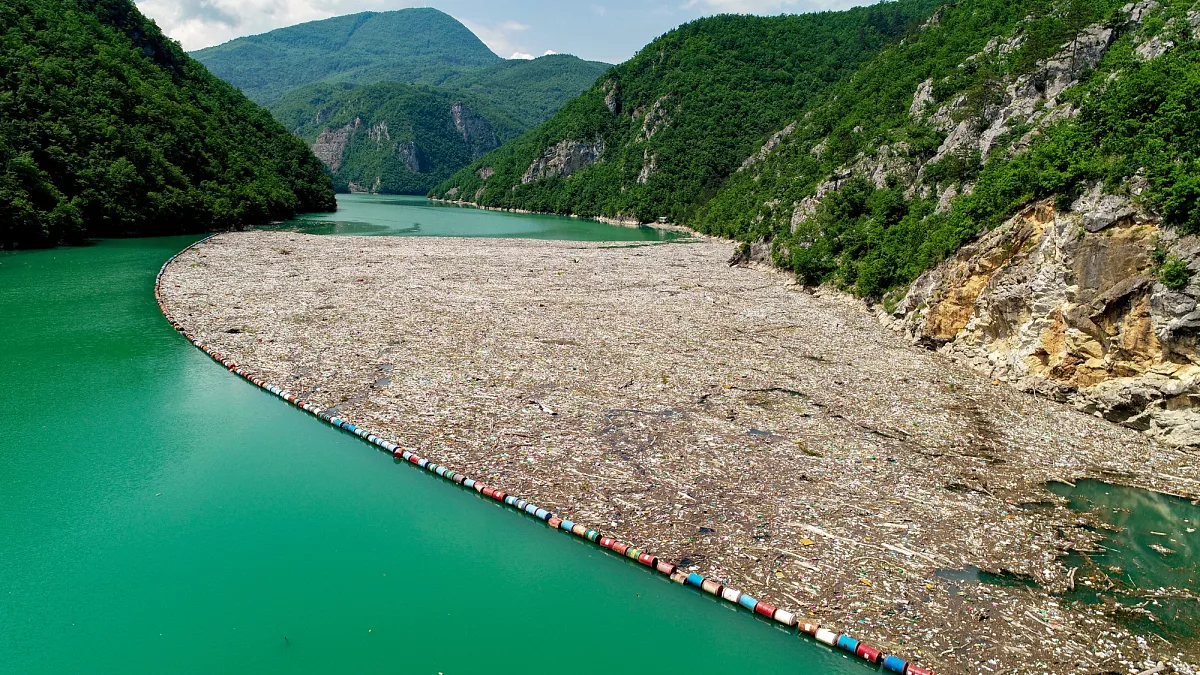
\includegraphics[width=0.6\textwidth,frame]{drina_waste}
	\caption{A drinai hulladéksziget. Egy lebegő zsinor fogja meg a műanyagpalackokat \cite{euronews2024}}
    \label{fig:drina-floating-waste}
\end{figure}

\begin{figure}[H]
	\centering
	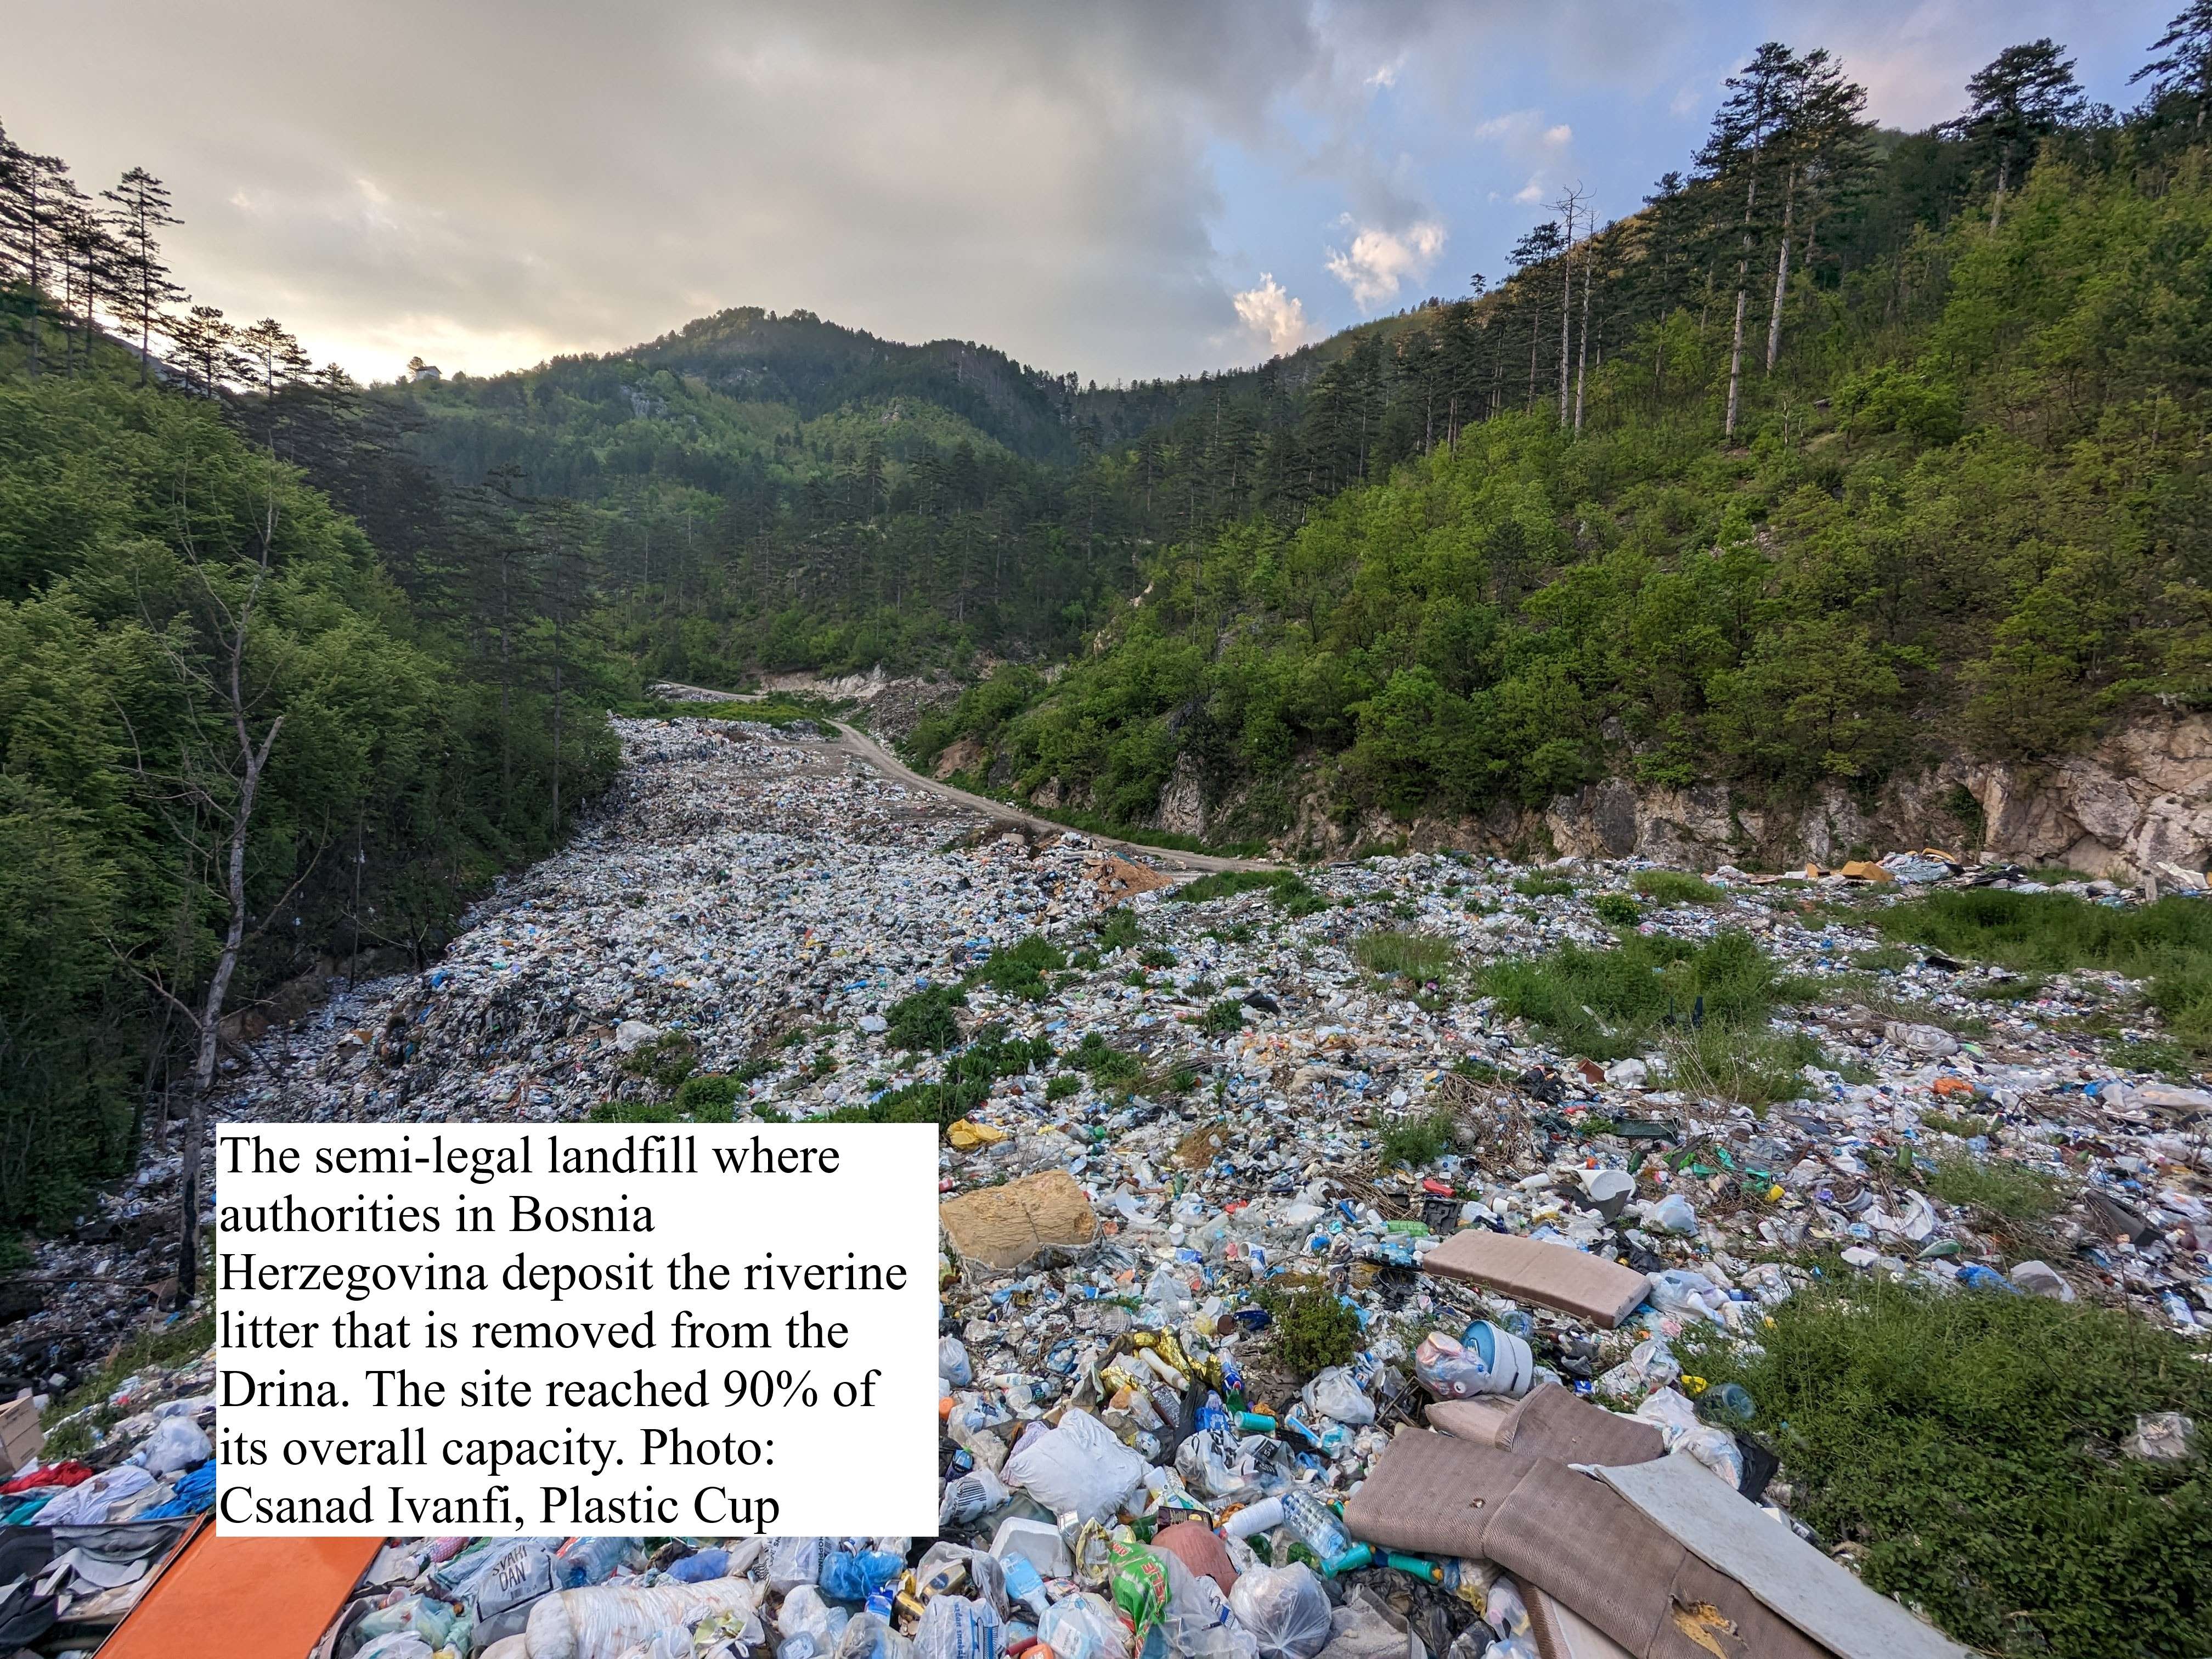
\includegraphics[width=0.6\textwidth,frame]{drina_deposit}
	\caption{A Drina melletti féllegális szemétlerakó \cite{petkupa2024}}
    \label{fig:drina-deposit}
\end{figure}

\begin{figure}[H]
	\centering
  \subcaptionbox{A teszthalmaz kézi annotációja}{
		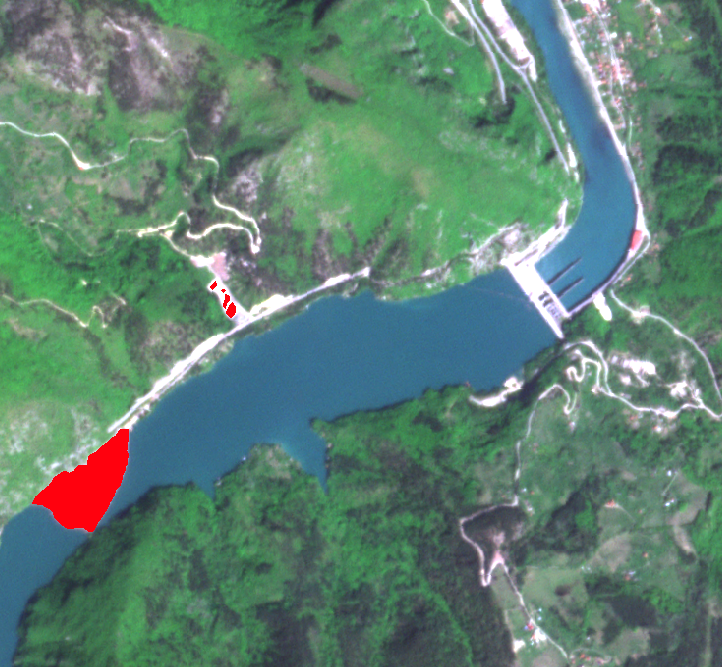
\includegraphics[width=0.45\linewidth]{drina-test}}
	\hspace{5pt}
	\subcaptionbox{A teszthalmaz annotációja a régi modellel}{
		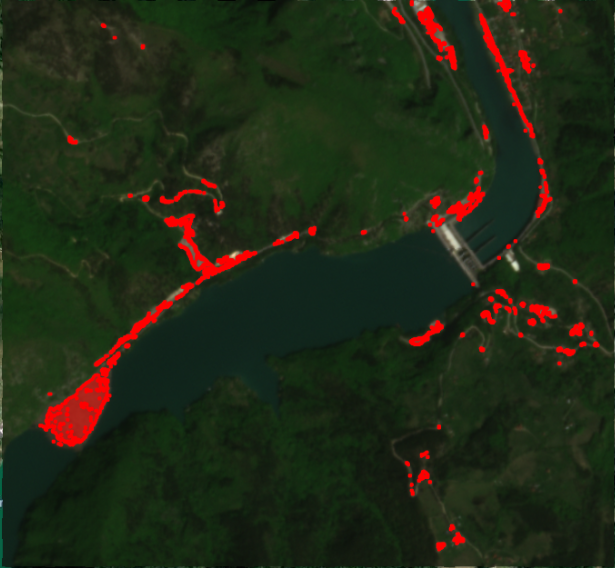
\includegraphics[width=0.45\linewidth]{drina-old}}
	\hspace{5pt}
	\subcaptionbox{A teszthalmaz annotációja az új modellel}{
		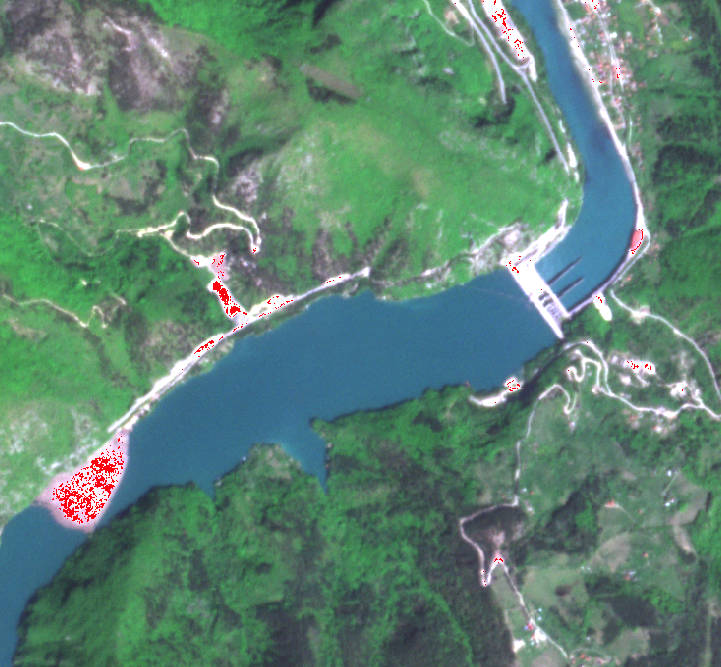
\includegraphics[width=0.45\linewidth]{drina-new}}
	\caption{Az új modell összehasonlítása a régi modellel az egyik Drinai teszt felvételen. Felvétel dátuma: 2023.05.07.}
	\label{fig:old-vs-new}
\end{figure}
\todo[color=blue!50]{Ez és a többi Drinás kép nagyon sötét. Jó lenne kicsit világosítani a hátteren, akár Photoshoppal :)}

\section{Teljesítmény mérése}

A teszthalmaz eredményeit a "Confusion Matrix" módszerével értékeltem ki \cite{CONGALTON199135}. Ezután ezeket az értékeket arra használtam, hogy a "Comission rate" (\ref{eq:comission-rate} képlet), "Omission rate" (\ref{eq:omission-rate} képlet), "Match rate" (\ref{eq:match-rate} képlet), illetve "Extraction rate" (\ref{eq:extraction-rate} képlet) értékeket számítsam ki \cite{Fekete2021}.

\begin{equation}\label{eq:comission-rate}
    Comission \ rate = \frac{N_{com}}{N_{ref}}
\end{equation}

\begin{equation}\label{eq:omission-rate}
    Omission \ rate = \frac{N_{om}}{N_{ext}}
\end{equation}

\begin{equation}\label{eq:match-rate}
    Match \ rate = \frac{N_{match}}{N_{ref}}
\end{equation}

\begin{equation}\label{eq:extraction-rate}
    Extraction \ rate = \frac{N_{ext}}{N_{ref}}
\end{equation}

$N_{com}$, $N_{om}$, $N_{match}$, $N_{ext}$, $N_{ref}$, rendre a false positive, false negative (A mátrix mellékátlói), true positive (A mátrix főátlója), a modell által detektált pozitív, illetve a referencia adatokban található positív értékek. Összehasonlítottam az új modell teljesítményét a régi modell teljesítményével. A \ref{tab:old-vs-new} táblázatból látható a két modell teljesítményének az átlaga a három felvételen.

\begin{table}[H]
	\centering
	\begin{tabular}{ | p{0.33\textwidth} | p{0.33\textwidth} | p{0.33\textwidth} | }
		\hline
		\textbf{Mérés azonosító} & \textbf{Régi modell átlagai (\%)} & \textbf{új modell átlagai (\%)} \\
		\hline \hline
		\emph{Comission Rate} & 63.67 & 28.13 \\
		\hline
		\emph{Omission Rate} & 26.21 & 70.67 \\
		\hline
		\emph{Match Rate} & 73.79 & 29.32 \\
		\hline
        \emph{Extraction Rate} & 208.18 & 41.31 \\
		\hline
	\end{tabular}
	\caption{A régi modell és az új modell teszteredményei átlagolva}
	\label{tab:old-vs-new}
\end{table}

Az új modell egy jóval kisebb false postive aránnyal rendelkezik mint a régi modell, de cserében a false-negative arányok is nagyok. Ennek oka a \ref{fig:old-vs-new} ábrából látható, hiszen a régi modell sokkal több pontot detektál a hulladékszigeten, míg az új modell kevesebb pontot detektál, de továbbra is nagy mértékben megtalálja a hulladékszigetet. Illetve a \ref{ch:test-set} fejezetben is tárgyaltam, hogy a szárazföldi hulladéklerakót a folyó mellett az új modell már megtalálja, míg a régi nem találja meg. Tekintve arra, hogy a match rate a true positive-al arányos, és az Extraction rate az összes pozitive-al arányos, ezek az értékek is kisebbek lesznek, mint a régi modell értékei.

\section{Főkomponens analízis teljesítménye}
\label{ch:pca-performance}

A \ref{ch:pca-methodology} fejezetben részletezett főkomponens analízis módszert is összehasonlítottam az új modell teljesítményével, a Confusion Matrix módszerének segítségével. A \ref{fig:pca-vs-no-pca} ábrából látható, hogy a főkomponens analízissel tanított modell sokkal jobban ki tudja szűrni a vízfelszínen kialakuló zajt. Az is látható, hogy a főkomponens analízissel kombinált Random Forest is hasonlóan tudja detektálni a hulladékkal szennyezett területeket, annyi különbséggel, hogy a hulladékos területen több pontot detektál, de cserében több false-positive-ot termel.

\begin{figure}[H]
	\centering
  \subcaptionbox{A teszthalmaz kézi annotációja}{
		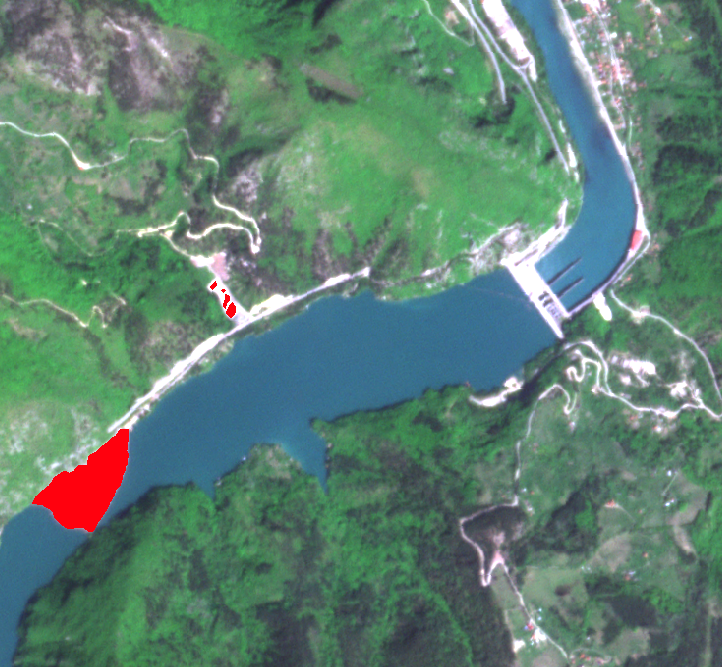
\includegraphics[width=0.45\linewidth]{drina-test}}
	\hspace{5pt}
	\subcaptionbox{A teszthalmaz annotációja az új modellel}{
		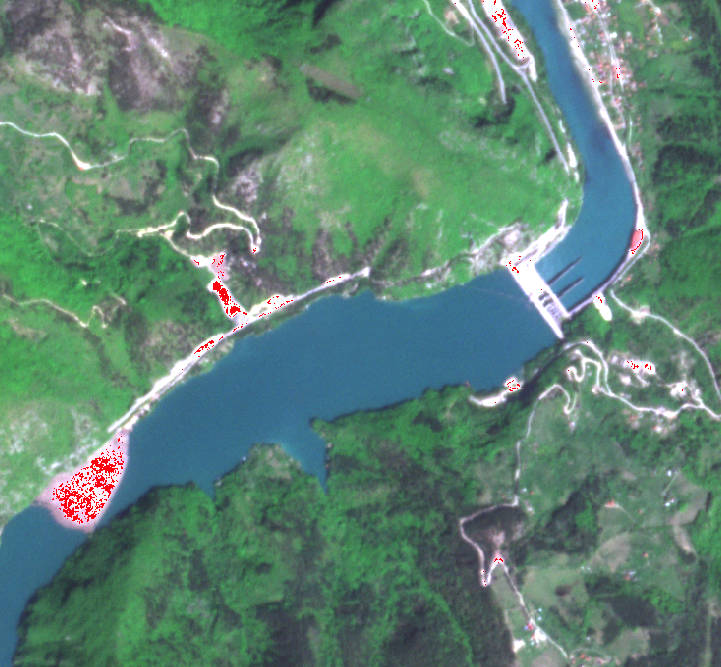
\includegraphics[width=0.45\linewidth]{drina-new}}
	\hspace{5pt}
	\subcaptionbox{A teszthalmaz annotációja az új modellel, PCA segítségével}{
		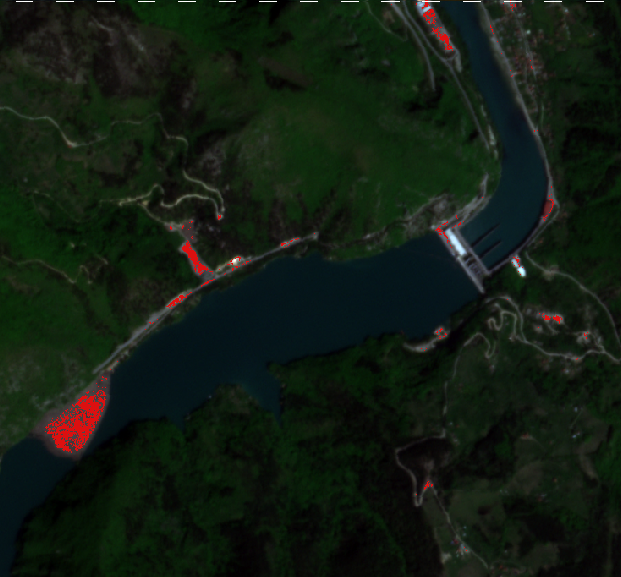
\includegraphics[width=0.45\linewidth]{drina-with-pca}}
	\caption{Az új modell összehasonlítása a PCA-val tanított modellel az egyik Drinai teszt felvételen. Felvétel dátuma: 2023.05.07.}
	\label{fig:pca-vs-no-pca}
\end{figure}

A \ref{tab:pca-vs-no-pca} táblázatban összesítem a főkomponens analízis mutatóit. A táblázatból leolvasható, hogy míg a főkomponens analízis picivel nagyobb false positive aránnyal rendelkezik, egyben kisebb false negative aránnyal rendelkezik. Ráadásul a felvételeken készülő zajt sokkal jobban kezeli, amint a \ref{fig:classification-pca-vs-no-pca} ábrából is látható: a piros jelöli a hulladékkal szennyezett területeket, kék jelöli a vizet, zöld jelöli a növényzettel borított területet, barna jelöli a mezőt és szürke jelöli az ismeretlen pixeleket, mint például épületek vagy utak. A főkomponens analízissel betanított modell sokkal jobban tudta detektálni a vizet a folyón, mint a főkomponens analízis nélküli modell.

\begin{table}[H]
	\centering
	\begin{tabular}{ | p{0.33\textwidth} | p{0.33\textwidth} | }
		\hline
		\textbf{Mérés azonosító} & \textbf{PCA-val tanított modell átlagai (\%)} \\
		\hline \hline
		\emph{Comission Rate} & 39.01 \\
		\hline
		\emph{Omission Rate} & 65.00 \\
		\hline
		\emph{Match Rate} & 34.99  \\
		\hline
        \emph{Extraction Rate} & 65.25 \\
		\hline
	\end{tabular}
	\caption{A főkomponens analízissel betanított modell teljesítményének az átlagai}
	\label{tab:pca-vs-no-pca}
\end{table}

\begin{figure}[H]
	\centering
  \subcaptionbox{Drina műholdfelvétele}{
		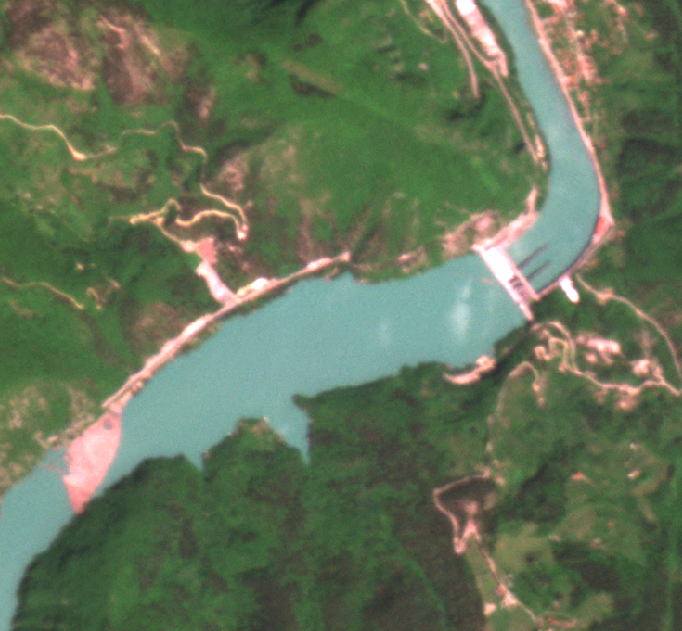
\includegraphics[width=0.45\linewidth]{drina20230521}}
	\hspace{5pt}
	\subcaptionbox{A PCA nélküli modell címkézése a Drinán}{
		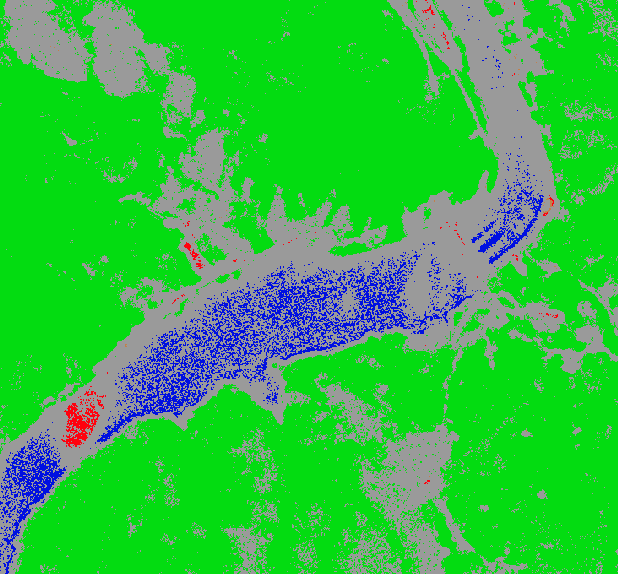
\includegraphics[width=0.45\linewidth]{drina-classification-no-pca}}
	\hspace{5pt}
	\subcaptionbox{A PCA-val betanított modell címkézése a Drinán}{
		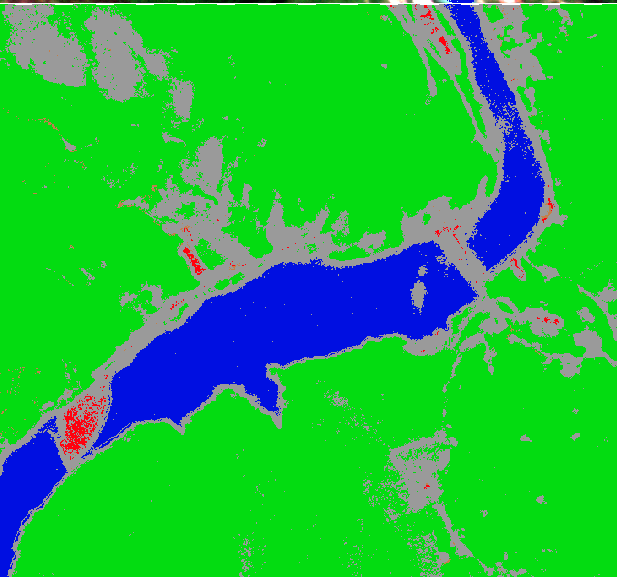
\includegraphics[width=0.45\linewidth]{drina-classification-with-pca}}
	\caption{A főkomponens analízissel betanított modell osztályozásának össszehasonlítása a PCA nélkül betanított modellel. Felvétel dátuma: 2023.05.21.}
	\label{fig:classification-pca-vs-no-pca}
\end{figure}

\section{Vízmaszkolás}
\todo[inline,color=blue!50]{A vízmaszkolásnak van egy műveleti költsége, így csak akkor fog megtérülni a használata, ha akkora területeket lehet kivágni vele, hogy jelentősen spórolunk azon, hogy azokon a területeken nem kell már hulladékot keresni. Emellett a víztől távoli false positive detektálások számát is tudja növelni.\\
Tamás töltött le egy nagyobb területet, talán ezt:\\
https://gis.inf.elte.hu:9000/ws-waste-detection/satellite\_images/manual/planetscope/Tisza-Szabolcs\\
Ezen kiértékelve milyen futási idő jön ki? Ha ott sem jó, akkor a hangsúlyt a false positive-ok csökkentésére helyezném, nem a teljesítményre.\\
Röviden érdemes a vízmaszkolásról írni szerintem, ha más nem, akkor a future work-ben.\\
Tamás munkáját nehéz hivatkozni, mivel nem adta / adja le ebben a félévben a diplomamunkáját. Ezen a ponton elég lesz annyi, hogy a vízmaszkolást nem te implementáltad, hanem a labor egy másik résztvevője.}

Az egyik kihívás a hulladékdetektálásban a nagy lefedettségű területek feldolgozása. A kutatásunk célja a folyók közelében található hulladékkal szennyezett területeknek a detektálása, így a folyóktól távolabbi területeket érdemes kivágni a gyorsabb osztályozás érdekében. Az egyik hosszútávú cél az, hogy hosszabb folyószakaszokon is lehessen futtatni a Random Forest modellt, úgy, hogy az osztályozás elfogadható futási időn belül történjen meg.
Ehhez használtam a vízmaszkolási algoritmust, amit a laboron belül elkészített az egyik kollégám, és megvizsgáltam a modell futási sebességét egy hosszú folyószakaszon. A \ref{tab:river-mask-performance} táblázatból látható, hogy a vízmaszkolás segítségével lényegesen fel lehet gyorsítani a feldolgozás sebességét.

\begin{table}[H]
	\centering
	\begin{tabular}{ | p{0.33\textwidth} | p{0.33\textwidth} | p{0.33\textwidth} | }
		\hline
		\textbf{Felvétel mérete (pixel)} & \textbf{folyó maszk nélküli futási idő} & \textbf{futási idő folyó maszkkal} \\
		\hline \hline
		 17520 * 13266 = 232,420,320 & 1 óra 41 perc & 2 óra 4 perc \\
		\hline
	\end{tabular}
	\caption{Folyó maszk nélküli futási idő összevetve a folyó maszkolásos futási idővel}
	\label{tab:river-mask-performance}
\end{table}

\section{Nyári és téli adatokra bontás teljesítménye}
\label{ch:summer-winter-models}

A nyári és téli adatokra bontásnál javulásra lehet számítani az eredményekben, tekintve arra, hogy a két modell az adott évszakokra specializálódik. A \ref{tab:summer-winter-split} táblázatból \todo{táblázatot kijavítani} látható, hogy a külön nyári felvételeken tanított modell jobban teljesít az általánosan betanított modellnél a nyári felvételeken, illetve a téli modell jobban teljesít az általánosan betanított modellnél a téli felvételeken. A \ref{fig:summer-vs-new} ábrából látható, hogy a nyári modell egy picivel jobban teljesít, mint az általános modell. Természetesen ebbe az irányba haladni azt az implikációt vonja maga után, hogy két modellt kell karbantartani egy modell helyett. Ugyanakkor a téli modell validálása külön kihívást jelent tekintve arra, hogy téli időszakban sokszor homályosak a felvételek a magasabb csapadékszint, és felhősebb viszonyok miatt, emiatt szabad szemmel nehezebb ellenőrizni a modell teljesítményét. Ennek fényében egy további lépése lehet a kutatásnak, hogy akár személyesen, akár magas felbontású drónfelvételek segítségével a téli felvételeket külön leellenőrizzük. 

\begin{table}[H]
	\centering
	\begin{tabular}{ | p{0.33\textwidth} | p{0.33\textwidth} | }
		\hline
		\textbf{Mérés azonosító} & \textbf{Nyári modell átlagai (\%)} \\
		\hline \hline
		\emph{Comission Rate} & 39.01 \\
		\hline
		\emph{Omission Rate} & 65.00  \\
		\hline
		\emph{Match Rate} & 34.99  \\
		\hline
        \emph{Extraction Rate} & 65.25 \\
		\hline
	\end{tabular}
	\caption{A külön nyári és téli időszakra tanított modellek átlagai}
	\label{tab:summer-winter-split}
\end{table}

\begin{figure}[H]
	\centering
  \subcaptionbox{A teszthalmaz kézi annotációja}{
		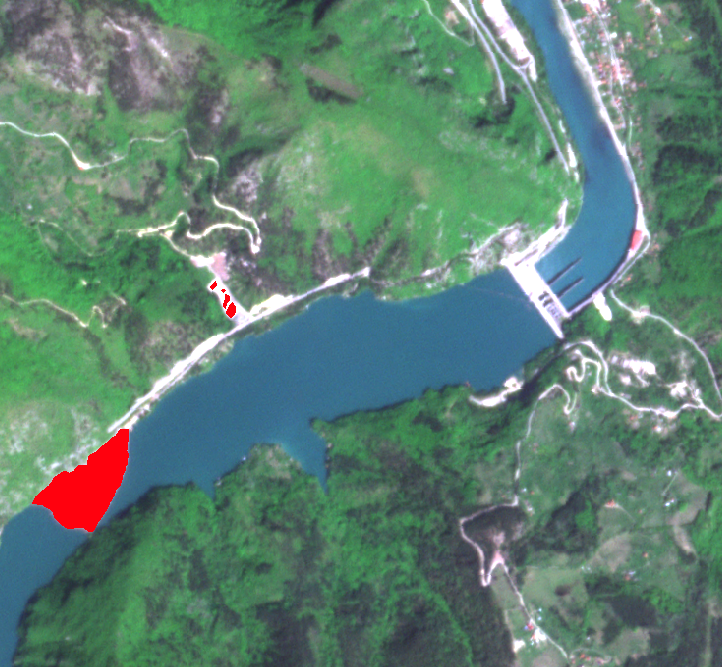
\includegraphics[width=0.45\linewidth]{drina-test}}
	\hspace{5pt}
	\subcaptionbox{A teszthalmaz annotációja az új modellel}{
		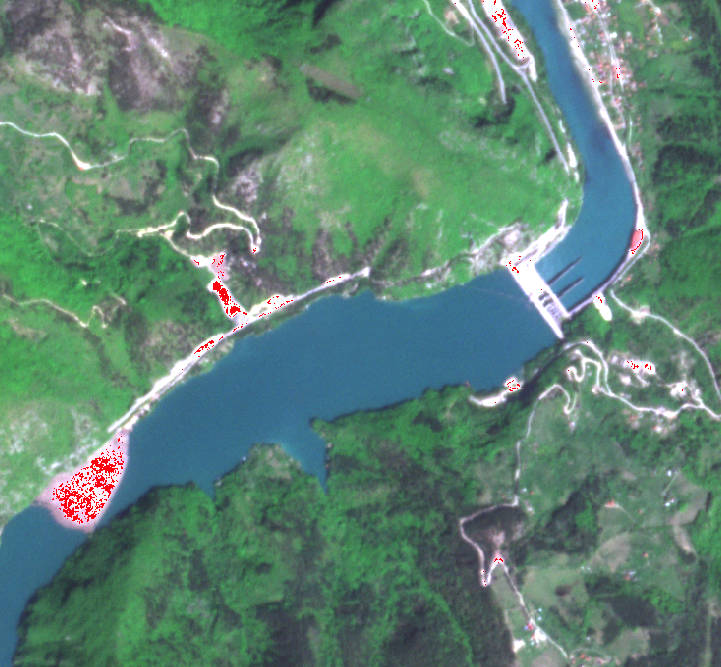
\includegraphics[width=0.45\linewidth]{drina-new}}
	\hspace{5pt}
	\subcaptionbox{A teszthalmaz annotációja a nyári modellel}{
		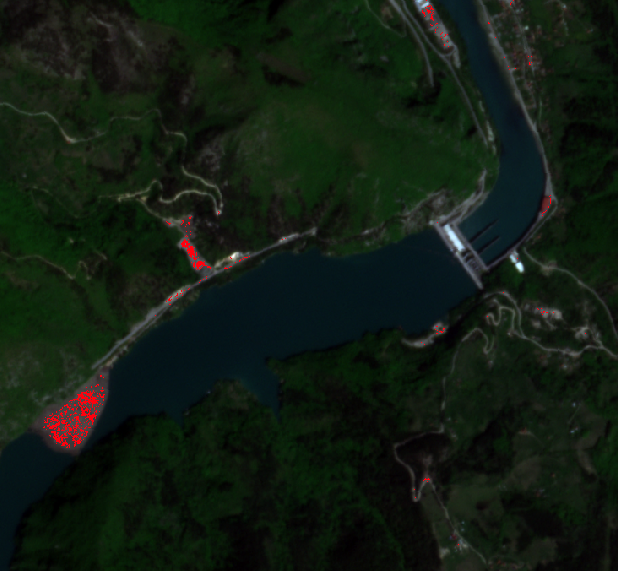
\includegraphics[width=0.45\linewidth]{drina-summer}}
	\caption{Az új modell összehasonlítása a nyári modellel az egyik Drinai teszt felvételen. Felvétel dátuma: 2023.05.07.}
	\label{fig:summer-vs-new}
\end{figure}

\section{Normalizálás tesztelése}
\label{ch:normalization-test} 

A normalizálásnak az volt a motivációja, hogy azokat a felvételeket, amik spektrális értékeikben lényeges eltéréseket tartalmaznak a többi felvételhez képest, tudjam értelmezhetővé tenni a modell számára. Teszteléshez kiválasztottam egy nyári Drinai felvételt, amin az új modell rosszul teljesített, és összehasonlítottam a normalizált képeken betanított modell eredményeivel. A \ref{fig:normal-vs-normalized-vs-old} ábrán látható, hogy a régi modell ezen a felvételen detektálta a hulladékszigetet, de vele együtt detektált nagyon sok false-positive-et is. Az új, normalizálás nélküli modell nagyon kevés hulladékot detektált, míg a normalizált modell ugyancsak sok false-positive-ot detektált. Habár első körben a normalizálással nem a várt eredményeket értem el, egy további kutatási irány lehet ennek a továbbvizsgálása, esetleg más referenciafelvételek megválasztása.

\begin{figure}[H]
	\centering
  \subcaptionbox{A régi modell teljesítménye}{
		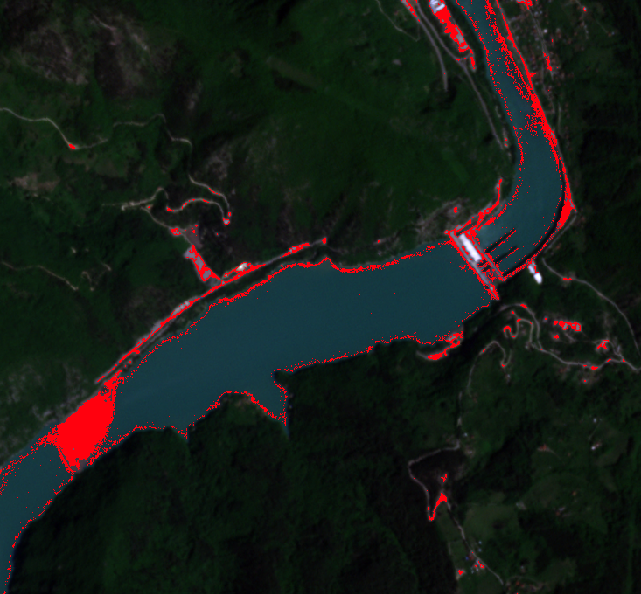
\includegraphics[width=0.45\linewidth]{drina-old-model-20230524}}
	\hspace{5pt}
	\subcaptionbox{Az új, normalizáció nélküli modell teljesítménye}{
		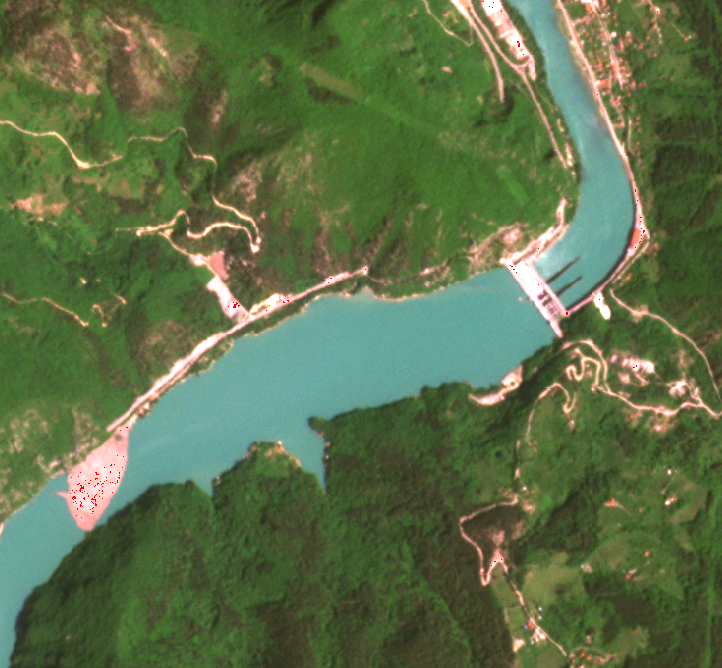
\includegraphics[width=0.45\linewidth]{drina-with-extra-unknowns-model-20230524}}
	\hspace{5pt}
	\subcaptionbox{Az új, normalizációval tanított modell teljesítménye}{
		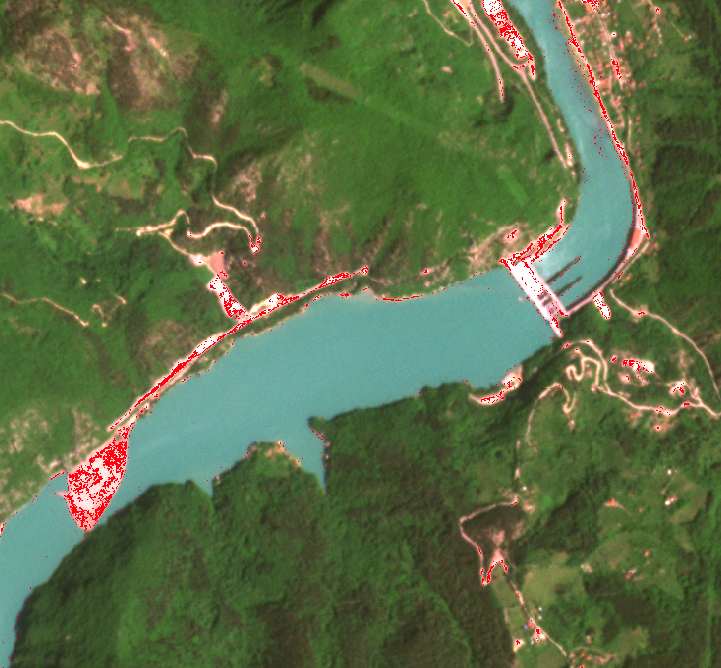
\includegraphics[width=0.45\linewidth]{drina-reference-model-20230524}}
	\caption{A régi, a normalizáció nélkül tanított és a normalizációval tanított modell összehasonlítása a Drinán. Felvétel dátuma: 2023.05.24.}
	\label{fig:normal-vs-normalized-vs-old}
\end{figure}


\section{Empirikus validáció}
\label{ch:empirical-validation}
Az empirikus validáció alá esnek a téli drinai és nyári kiskörei felvételek. Ennek az az oka, hogy a téli drinai felvételek közül kihívás volt megfelelő minőségű felvételt találni numerikus validációra, míg a 2023-as kiskörei adathalmaz tanításra volt használva, így a 2024-es adathalmazból való felvételek is alkalmatlannak bizonyultak numerikus validációra. 

A \ref{fig:drina-winter-all-models} ábrából látható, hogy a téli felvételen árnyék takarja a hulladéksziget felét. Itt látszik, hogy a modellek számára kihívást jelent az árnyék alatt levő hulladéksziget detektálása. Az egyetlen modell, aki képes volt detektálni az árnyék alatti szigetet, az a régi modell volt, de cserében nagyon sok false-positive-ot termelt a többi modellhez képest. Így, a kutatás jelenlegi állapotában a téli hulladékdetektálás jelenti az egyik nagy kihívást.

A \ref{fig:kiskore-all-models} ábrán egy kiskörei felvételen hasonlítottam össze az összes modellt. A három legjobban teljesítő modell az új modell, a nyári adatokon betanított új modell, illetve a főkomponens analízissel betanított modell. Míg a nyári adatokon tanított modell közel teljesített az új modellhez képest, a főkomponens analízissel betanított modell több területet hulladékosnak jelölt a szeméttorlaszon, de cserében intenzívebbek is voltak a false-positive értékek.

\begin{figure}[H]
	\centering
  \subcaptionbox{A teszthalmaz kézi annotációja}{
		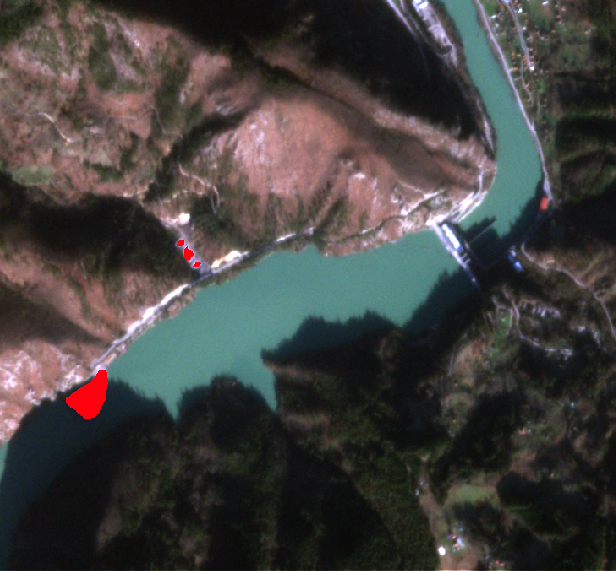
\includegraphics[width=0.45\linewidth]{drina-test-20231217}}
	\hspace{5pt}
	\subcaptionbox{A teszthalmaz annotációja a régi modellel}{
		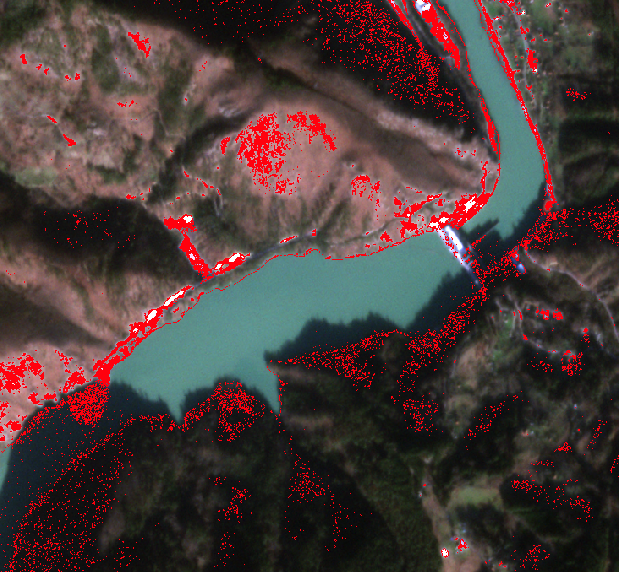
\includegraphics[width=0.45\linewidth]{drina-old-20231217}}
	\hspace{5pt}
	\subcaptionbox{A teszthalmaz annotációja az új modellel}{
		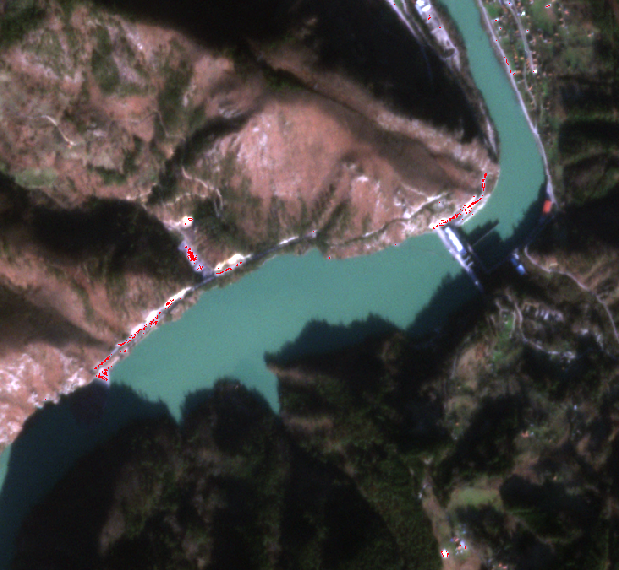
\includegraphics[width=0.45\linewidth]{drina-new-20231217}}
	\hspace{5pt}
	\subcaptionbox{A teszthalmaz annotációja a téli modellel}{
		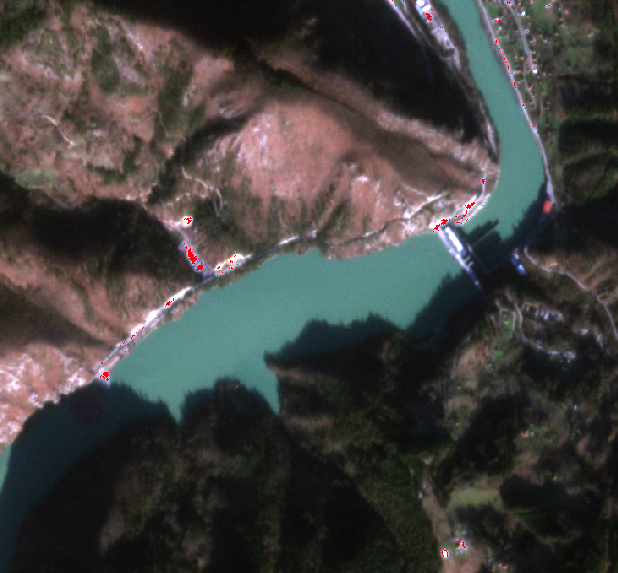
\includegraphics[width=0.45\linewidth]{drina-winter-20231217}}
	\hspace{5pt}
	\subcaptionbox{A teszthalmaz annotációja a normalizált modellel}{
		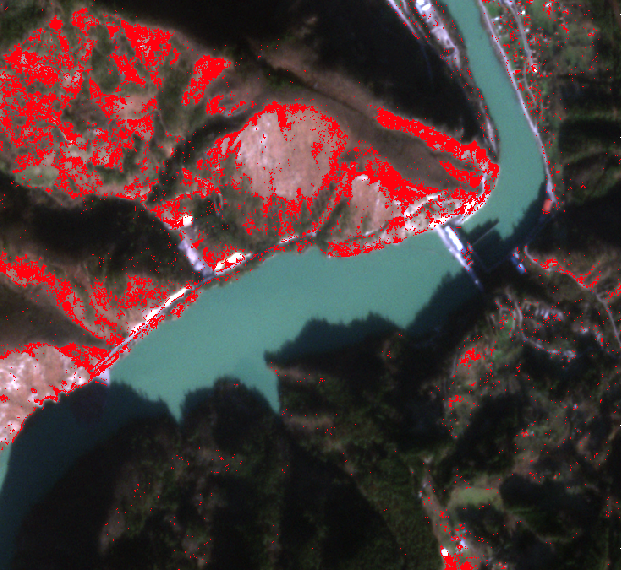
\includegraphics[width=0.45\linewidth]{drina-reference-20231217}}
	\hspace{5pt}
	\subcaptionbox{A teszthalmaz annotációja a PCA-val tanított modellel}{
		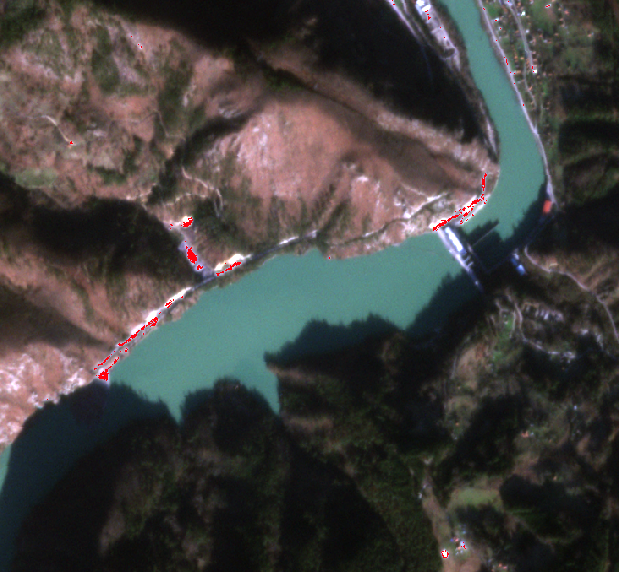
\includegraphics[width=0.45\linewidth]{drina-pca-20231217}}
	\caption{Az összes modell összehasonlítása az egyik téli drinai teszt felvételen. Felvétel dátuma: 2023.12.17.}
	\label{fig:drina-winter-all-models}
\end{figure}

\begin{figure}[H]
	\centering
  \subcaptionbox{A teszthalmaz kézi annotációja}{
		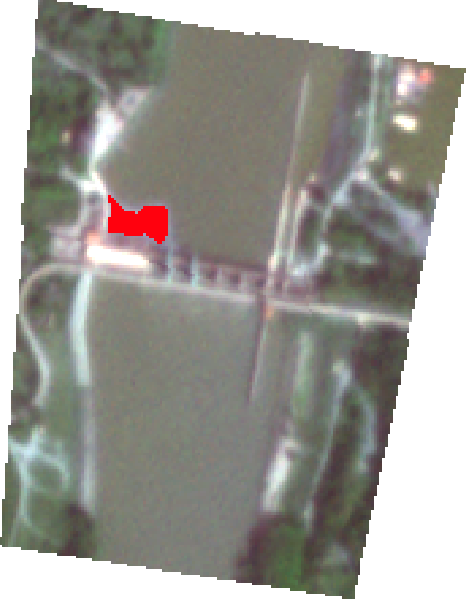
\includegraphics[width=0.30\linewidth]{kiskore-test-20240412}}
	\hspace{5pt}
	\subcaptionbox{A teszthalmaz annotációja a régi modellel}{
		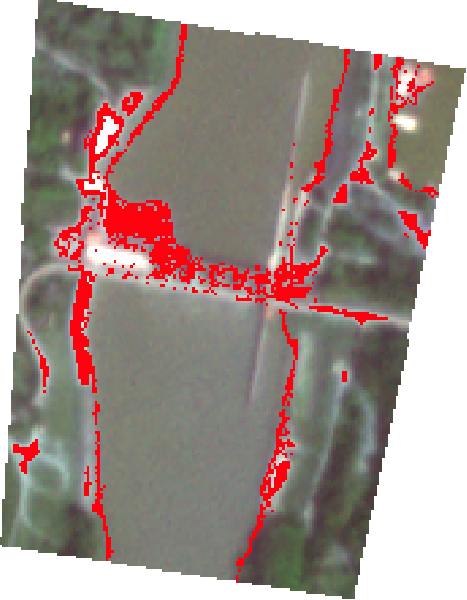
\includegraphics[width=0.30\linewidth]{kiskore-old-20240412}}
	\hspace{5pt}
	\subcaptionbox{A teszthalmaz annotációja az új modellel}{
		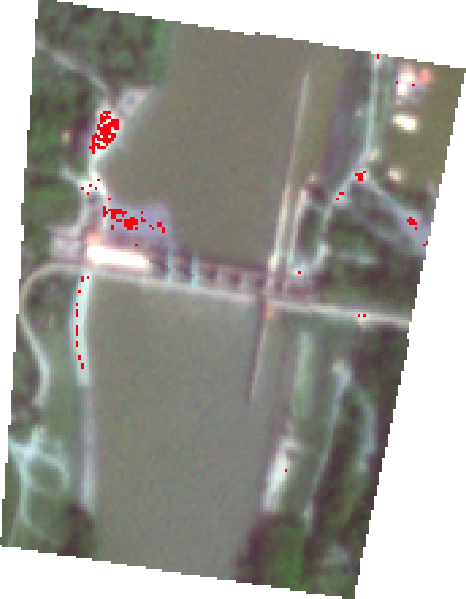
\includegraphics[width=0.30\linewidth]{kiskore-new-20240412}}
	\hspace{5pt}
	\subcaptionbox{A teszthalmaz annotációja a nyári modellel}{
		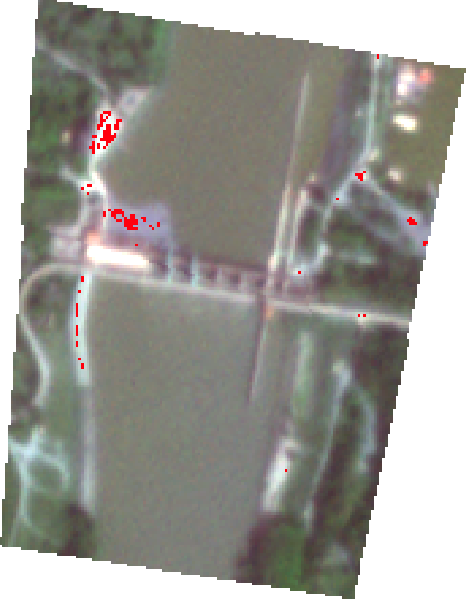
\includegraphics[width=0.30\linewidth]{kiskore-summer-20240412}}
	\hspace{5pt}
	\subcaptionbox{A teszthalmaz annotációja a normalizált modellel}{
		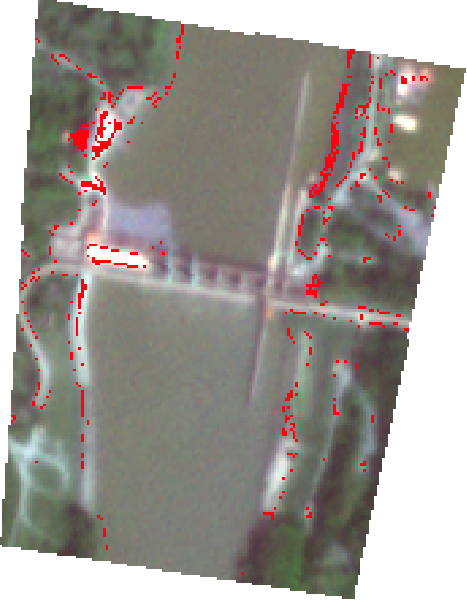
\includegraphics[width=0.30\linewidth]{kiskore-reference-20240412}}
	\hspace{5pt}
	\subcaptionbox{A teszthalmaz annotációja a PCA-val tanított modellel}{
		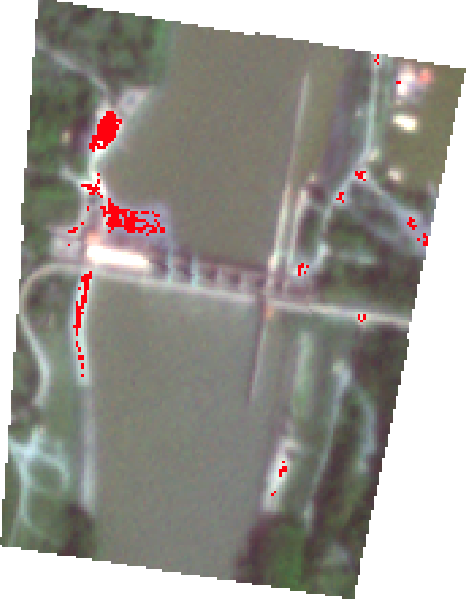
\includegraphics[width=0.30\linewidth]{kiskore-pca-20240412}}
	\caption{Az összes modell összehasonlítása az egyik kiskörei teszt felvételen. Felvétel dátuma: 2024.04.12.}
	\label{fig:kiskore-all-models}
\end{figure}